\section{Simulations and Numerical Experiments}

We conducted evolutionary Prisoner’s Dilemma simulations on both networks, varying the initial state of Bernoulli for the starting strategies \(p \in \{0.25, 0.50, 0.75\}\). For each combination of network and \(p\), we compared two standard payoff‐based update rules (imitate‐best‐neighbor and Fermi). Then for every combination of the Epinions' data set, we compared the trust update rules (trust aware update and all neighbor trust).  In every experiment, we recorded the final fraction of cooperators and the number of iterations required for the dynamics to converge.


\subsection{Intuition}
Prior to conducting our simulations, we formulated the following expectations. First, we hypothesized that under standard payoff‐based update rules (imitate‐best‐neighbor and Fermi), the dense, highly clustered Facebook network would sustain higher levels of cooperation than the sparser, more hierarchical Epinions network. Second, we expected that introducing trust-awareness into the update process would uniformly boost cooperative behavior. Finally, we expected that an all‐neighbor trust aggregation rule—by leveraging the full spectrum of positive and negative ties—would produce the most robust and rapid convergence to cooperation across both network topologies.


\section{Results}

\begin{landscape}
\begin{table}[p]
  \centering
  % Use the smallest readable font:
  \tiny
  \caption{“Cooperator (\%) vs.\ Iteration” plots, final‐split percentages, and iterations to convergence, organized by update rule.}
  \label{tab:fb_ep_compact_final}
  \vspace{0.5em}

  % Define a very narrow column type “S” for Final‐Split cells
  \newcolumntype{S}{>{\centering\arraybackslash}m{0.8cm}}
  % Define a very wide column type “P” for plot cells
  \newcolumntype{P}{>{\centering\arraybackslash}m{3.4cm}}

  % Tighten spacing between columns
  \setlength{\tabcolsep}{2pt}

  % Define the new, mixed table structure: S-S-S-P for FB, P-S-S-S for EP
  \begin{tabular}{%
      l | S S S P | P S S S | P S S S
    }
    \toprule
    % Row 1: Dataset
    & \multicolumn{4}{c|}{\bfseries Facebook}
    & \multicolumn{8}{c}{\bfseries Epinion} \\
    \cmidrule(lr){2-5} \cmidrule(lr){6-13}

    % Row 2: Game Type
    {\bfseries Update Rule}
    & \multicolumn{4}{c|}{\bfseries Std. Game}
    & \multicolumn{4}{c|}{\bfseries Std. Game}
    & \multicolumn{4}{c}{\bfseries Trust-Aware} \\
    \cmidrule(lr){2-5} \cmidrule(lr){6-9} \cmidrule(lr){10-13}

    % Row 3: Header for split percentages and convergence iterations
    & \multicolumn{3}{c|}{\bfseries\shortstack{Cooperate \% \\[-0.3em] Defect \% \\[-0.3em] (Conv. Iter.)}} & {\bfseries Plot}
    & {\bfseries Plot} & \multicolumn{3}{c|}{\bfseries\shortstack{Cooperate \% \\[-0.3em] Defect \% \\[-0.3em] (Conv. Iter.)}}
    & {\bfseries Plot} & \multicolumn{3}{c}{\bfseries\shortstack{Cooperate \% \\[-0.3em] Defect \% \\[-0.3em] (Conv. Iter.)}} \\
    \cmidrule(lr){2-4} \cmidrule(lr){7-9} \cmidrule(lr){11-13}

    % Row 4: p-values
    & {\(p=0.25\)} & {\(p=0.50\)} & {\(p=0.75\)} &
    & & {\(p=0.25\)} & {\(p=0.50\)} & {\(p=0.75\)}
    & & {\(p=0.25\)} & {\(p=0.50\)} & {\(p=0.75\)} \\
    \midrule

    Imitate–Best–Neighbor
      % Facebook Std. Game (S-S-S-P)
      & \shortstack{0.00\%\\100.00\%\\(3)} & \shortstack{77.25\%\\22.75\%\\(5)} & \shortstack{95.79\%\\4.21\%\\(5)}
      & 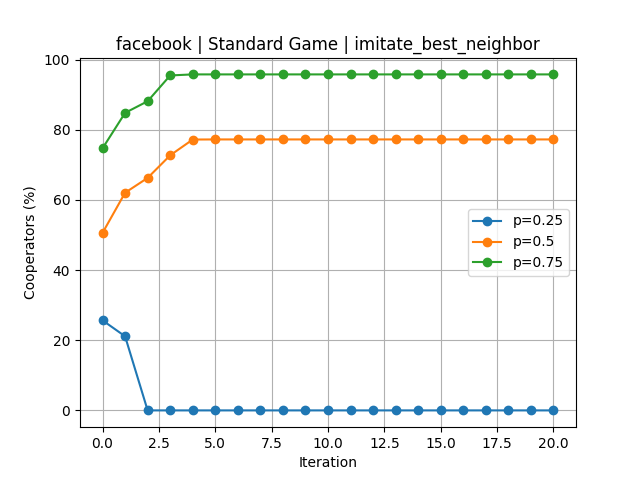
\includegraphics[width=3.4cm]{figures/plots/facebook_evolutionary_game_round_imitate_best_neighbor.png}
      % Epinion Std. Game (P-S-S-S)
      & 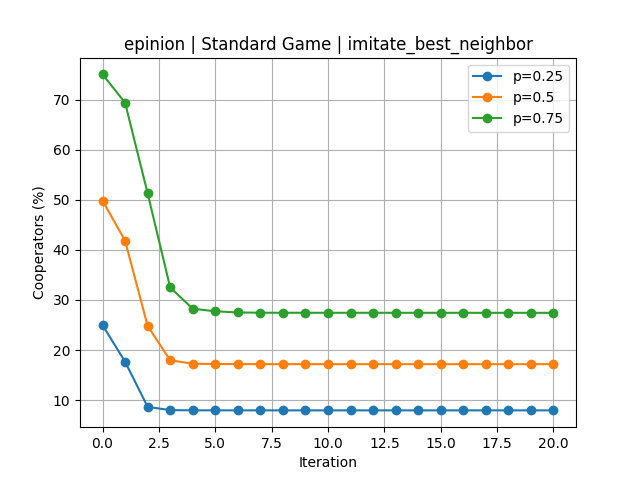
\includegraphics[width=3.4cm]{figures/plots/epinion_evolutionary_game_round_imitate_best_neighbor.png}
      & \shortstack{7.95\%\\92.05\%\\(4)} & \shortstack{17.18\%\\82.82\%\\(6)} & \shortstack{27.43\%\\72.57\%\\(8)}
      % Epinion Trust-Aware Game (P-S-S-S)
      & 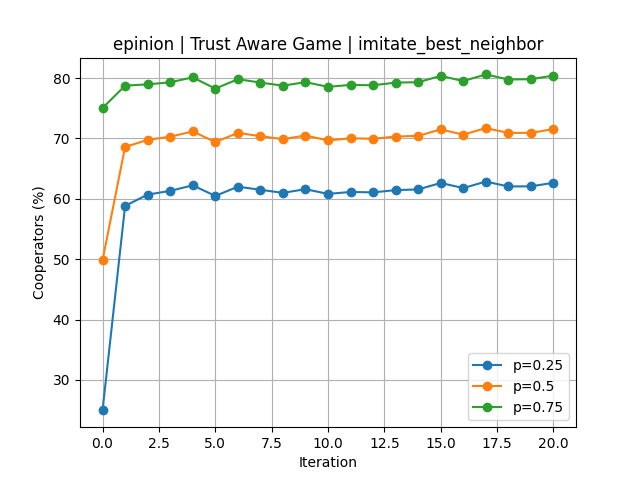
\includegraphics[width=3.4cm]{figures/plots/epinion_game_round_trust_imitate_best_neighbor.png}
      & \shortstack{62.66\%\\37.34\%\\(19)} & \shortstack{71.55\%\\28.45\%\\(19)} & \shortstack{80.42\%\\19.58\%\\(20)}
      \\[0.6em]

    Fermi–Update
      % Facebook Std. Game (S-S-S-P)
      & \shortstack{1.51\%\\98.49\%\\(10)} & \shortstack{5.89\%\\94.11\%\\(7)} & \shortstack{5.94\%\\94.06\%\\(17)}
      & 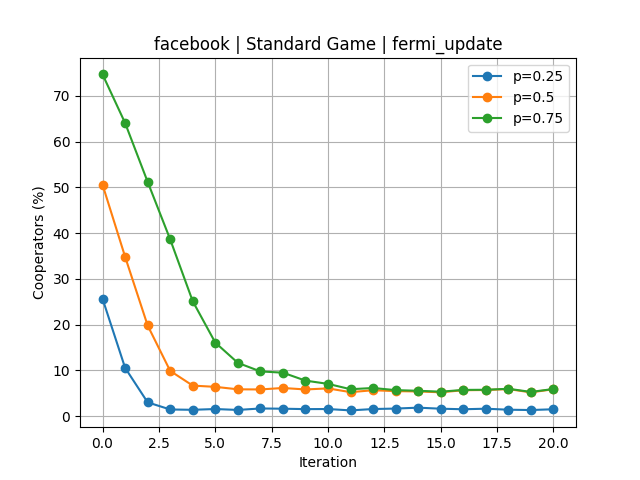
\includegraphics[width=3.4cm]{figures/plots/facebook_evolutionary_game_round_fermi_update.png}
      % Epinion Std. Game (P-S-S-S)
      & 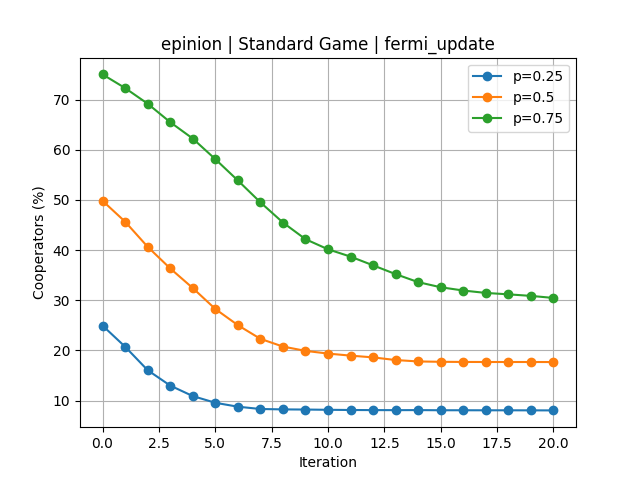
\includegraphics[width=3.4cm]{figures/plots/epinion_evolutionary_game_round_fermi_update.png}
      & \shortstack{8.05\%\\91.95\%\\(9)} & \shortstack{17.69\%\\82.31\%\\(16)} & \shortstack{30.47\%\\69.53\%\\(20)}
      % Epinion Trust-Aware Game (P-S-S-S)
      & 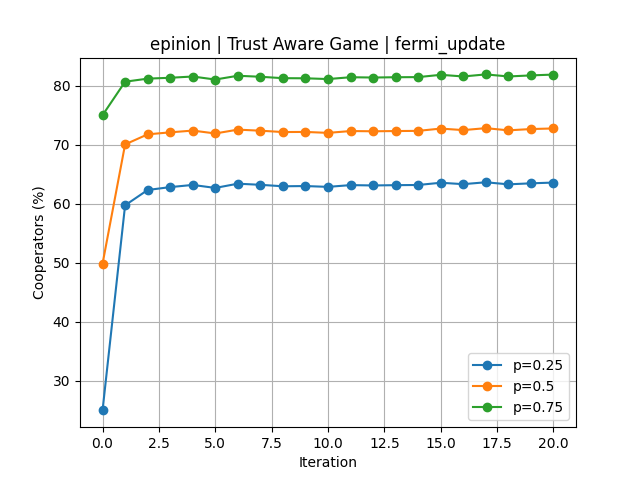
\includegraphics[width=3.4cm]{figures/plots/epinion_game_round_trust_fermi_update.png}
      & \shortstack{63.61\%\\36.39\%\\(9)} & \shortstack{72.79\%\\27.21\%\\(9)} & \shortstack{81.93\%\\18.07\%\\(9)}
      \\[0.6em]

    Trust–Aware–Update
      % Facebook Std. Game (N/A, S-S-S-P)
      & \shortstack{N/A\\N/A\\N/A} & \shortstack{N/A\\N/A\\N/A} & \shortstack{N/A\\N/A\\N/A}
      & \shortstack{N/A}
      % Epinion Std. Game (P-S-S-S)
      & 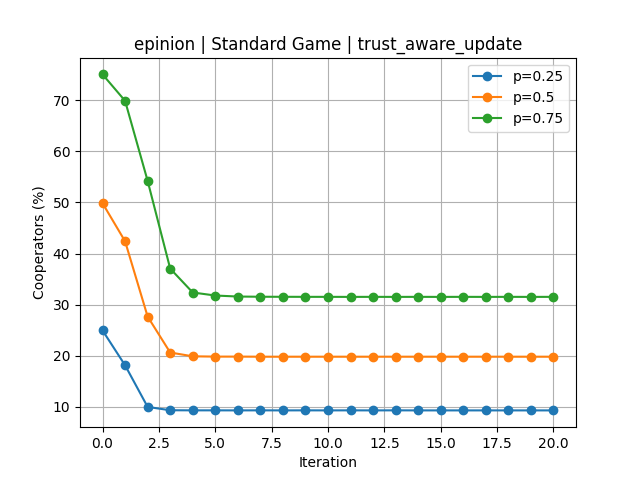
\includegraphics[width=3.4cm]{figures/plots/epinion_evolutionary_game_round_trust_aware_update.png}
      & \shortstack{9.32\%\\90.68\%\\(4)} & \shortstack{19.82\%\\80.18\%\\(6)} & \shortstack{31.53\%\\68.47\%\\(7)}
      % Epinion Trust-Aware Game (P-S-S-S)
      & 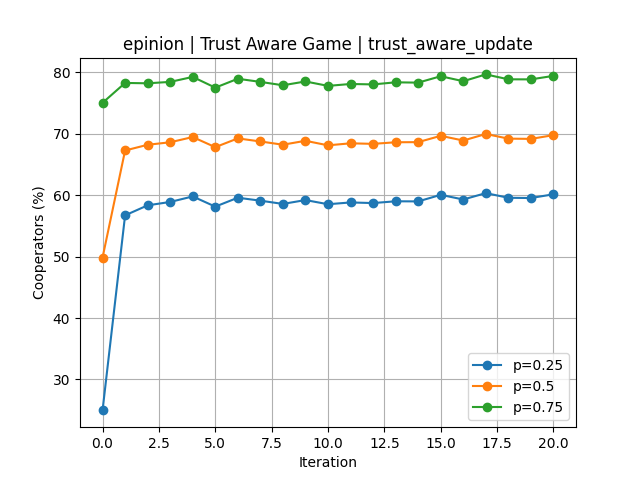
\includegraphics[width=3.4cm]{figures/plots/epinion_game_round_trust_trust_aware_update.png}
      & \shortstack{60.15\%\\39.85\%\\(14)} & \shortstack{69.78\%\\30.22\%\\(14)} & \shortstack{79.43\%\\20.57\%\\(14)}
      \\[0.6em]

    All–Neighbor–Trust
      % Facebook Std. Game (N/A, S-S-S-P)
      & \shortstack{N/A\\N/A\\N/A} & \shortstack{N/A\\N/A\\N/A} & \shortstack{N/A\\N/A\\N/A}
      & \shortstack{N/A}
      % Epinion Std. Game (P-S-S-S)
      & 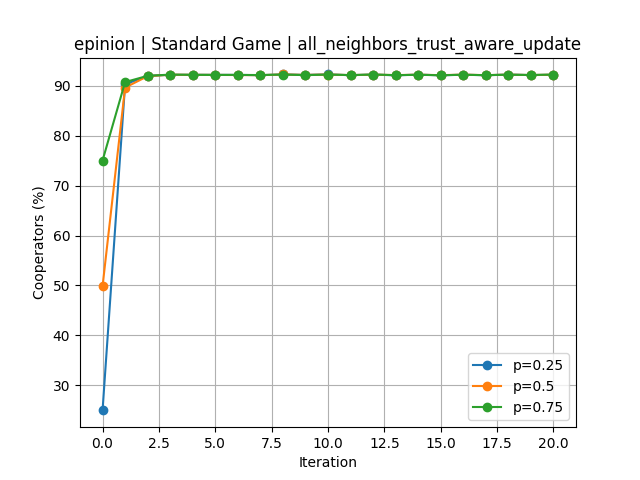
\includegraphics[width=3.4cm]{figures/plots/epinion_evolutionary_game_round_all_neighbors_trust_aware_update.png}
      & \shortstack{92.24\%\\7.76\%\\(4)} & \shortstack{92.25\%\\7.75\%\\(4)} & \shortstack{92.27\%\\7.73\%\\(4)}
      % Epinion Trust-Aware Game (P-S-S-S)
      & 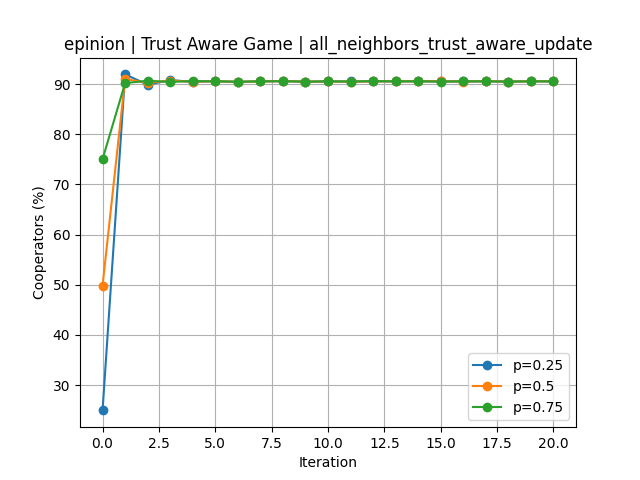
\includegraphics[width=3.4cm]{figures/plots/epinion_game_round_trust_all_neighbors_trust_aware_update.png}
      & \shortstack{90.54\%\\9.46\%\\(8)} & \shortstack{90.57\%\\9.43\%\\(8)} & \shortstack{90.57\%\\9.43\%\\(7)}
      \\

    \bottomrule
  \end{tabular}
\end{table}
\end{landscape}

\subsection{Cooperation Levels}
Table~I presents the final fraction of cooperators under three temptation parameters \(p\) for both the Facebook and Epinions networks across five update rules. Under standard \emph{imitate‐best‐neighbor}, Facebook transitions from 0\% cooperation at \(p=0.25\) to 95.8\% at \(p=0.75\), whereas Epinions peaks at only 27.4\%. The Fermi rule yields similar behavior: Facebook reaches 94\% cooperation at high \(p\), while Epinions remains below 31\%. When we apply trust‐aware versions of both imitation and Fermi updates on Epinions, final cooperation rises sharply into the 62–82\% range across all \(p\). Finally, the all‐neighbor‐trust rule drives cooperation above 90\% on Epinions irrespective of \(p\), demonstrating near‐universal cooperation under trust-aware updates.

\subsection{Convergence Speed}
Standard update rules on Epinions require up to 20 iterations to stabilize, reflecting slow cluster formation on its sparse topology. In contrast, trust update rules including both pairwise trust updates and the all‐neighbor‐trust converge in under 10 iterations (often within 5–8), highlighting trust’s ability to accelerate consensus. Facebook’s dense structure enables faster convergence under standard rules (3–5 iterations). 


